\documentclass[
11pt, % The default document font size, options: 10pt, 11pt, 12pt
oneside, % Two side (alternating margins) for binding by default, uncomment to switch to one side
english, % ngerman for German
singlespacing, % Single line spacing, alternatives: onehalfspacing or doublespacing
%draft, % Uncomment to enable draft mode (no pictures, no links, overfull hboxes indicated)
%nolistspacing, % If the document is onehalfspacing or doublespacing, uncomment this to set spacing in lists to single
%liststotoc, % Uncomment to add the list of figures/tables/etc to the table of contents
%toctotoc, % Uncomment to add the main table of contents to the table of contents
%parskip, % Uncomment to add space between paragraphs
%nohyperref, % Uncomment to not load the hyperref package
headsepline, % Uncomment to get a line under the header
chapterinoneline, % Uncomment to place the chapter title next to the number on one line
%consistentlayout, % Uncomment to change the layout of the declaration, abstract and acknowledgements pages to match the default layout
]{MastersDoctoralThesis} % The class file specifying the document structure


\usepackage[utf8]{inputenc} % Required for inputting international characters
\usepackage[T1]{fontenc} % Output font encoding for international characters
\usepackage{todonotes}
\usepackage{mathpazo} % Use the Palatino font by default
\usepackage{adjustbox} % Resize table
\usepackage[backend=bibtex,style=numeric-comp,sorting=none,natbib=true]{biblatex} % Use the bibtex backend with the authoryear citation style (which resembles APA)
\addbibresource{thesis.bib} % The filename of the bibliography
\usepackage{float}
\usepackage{graphicx}
\usepackage{rotating}
\usepackage[autostyle=true]{csquotes} % Required to generate language-dependent quotes in the bibliography
\usepackage{glossaries}
\usepackage[T1]{fontenc}
\usepackage{comment}
\usepackage{hyperref}
\makeglossaries
\loadglsentries{glossary}


\newcommand{\vgp}{\textsc{vgpop }}
\author{Flavia Villani, Vincenza Colonna}
\date{1 June 2020}

\begin{document}
\begin{titlepage}
\centering
{\scshape\large\normalfont\bfseries UNIVERSITÀ DEGLI STUDI DI NAPOLI FEDERICO II \par}
 \vspace{0.7cm} 
{\scshape\large\normalfont Dipartimento di Medicina Molecolare e 

Biotecnologie Mediche
 \vspace{0.7cm} 
 
 
 
\includegraphics[width=0.25\textwidth]{fig/logo.png}
 \par
 \vspace{0.5cm}
\hspace{2cm}
 \par}
 \vspace{0.2cm}
{\scshape\large\normalfont CORSO DI LAUREA MAGISTRALE IN 

BIOTECNOLOGIE MEDICHE
 \par}
 \vspace{0.5cm} 
{\scshape\large\normalfont TESI DI LAUREA SPERIMENTALE
 \par}
  \vspace{0.5cm}
%{\scshape\large\normalfont\bfseries\textit Statistical analysis of selection using pangenomics data models
 %\par}
{\scshape\large\normalfont\bfseries\textit \textit{vgpop}, a Python library for population genomics analyses from pangenomes
 \par}  

{\scshape\large\normalfont\bfseries\textit Population genomics analyses from pangenomes
 \par}  


  \vspace{0.8cm}
{\scshape\large\normalfont\bfseries   Analisi statistiche per la selezione usando dati pangenomici
 \par} 
\vspace{1cm} 
\begin{minipage}{0.45\textwidth}
{\scshape\normalfont\large\bfseries Relatore:}\\
{\scshape\normalfont\large Dott. Vincenza Colonna} \\ 
{\scshape\normalfont\large\bfseries Relatore interno:} \\
{\scshape\normalfont\large Ch.mo Prof. Gabriella De Vita}\\
{\scshape\normalfont\large\bfseries Correlatore:} \\
{\scshape\normalfont\large Dott. Erik Garrison}
\end{minipage}
\hspace{2.5cm}
\begin{minipage}{0.25\textwidth}
{\scshape\normalfont\large\bfseries Candidato:}\\
 {\scshape\normalfont\large Flavia Villani \\
 matr. N79001438} 
\end{minipage}

\vfill
\centering
\vspace{0.48cm} 
{\scshape\Large\normalfont A.A. 2019/2020}

\end{titlepage}
%\maketitle
%----------------------------------------------------------------------------------------
%	LIST OF CONTENTS/FIGURES/TABLES PAGES
%----------------------------------------------------------------------------------------

\tableofcontents % Prints the main table of contents

%\listoffigures % Prints the list of figures

%\listoftables % Prints the list of tables


%--------------------------------------------------------------------------------------

% Chapter discussion

\chapter{Abstract-1pagina}
    
 % Main chapter title

\label{Chapter0} % For referencing the chapter elsewhere, use \ref{Chapter4} 

%----------------------------------------------------------------------------------------

% Define some commands to keep the formatting separated from the content 
\newcommand{\keyword}[1]{\textbf{#1}}
\newcommand{\tabhead}[1]{\textbf{#1}}
\newcommand{\code}[1]{\texttt{#1}}
\newcommand{\file}[1]{\texttt{\bfseries#1}}
\newcommand{\option}[1]{\texttt{\itshape#1}}

%~~~~~~~~~~~~~~~~~~~~~~~~~~~~~~~~~~~~~~~~~~~~~~~~~~~~~~~~~~~~~~~~~~~~~~~~~~~~~~~~~~~~~~~
Studies of genomic selection typically assume a single linear reference genome. However, structural and complex variation can render this simplified model inapplicable. To address this limitation, during my thesis I started the development of a software library for the statistical analysis of negative selection using pangenomic data models. Typically represented in the Graphical Fragment Assembly (GFA) file format, these models represent whole genome alignments in a compact structure, without loosing information. Because a pangenome embeds the linear genomes from which it is constructed, we can choose a particular reference genome and project the variants on it. """ DIRE CHE E' RAPPRESENTATO COME UN GRAFO E POI CHE LE ZONE CONTENENTI VARIANTI APPAIONO COME BOLLE(which appear as bubbles in the graph)""". Therefore, I focused on develop algorithms for bubble detection, genereting Variant Call Format (VCF) files directly from graphs.\\

\noindent
We can use this variants projection to drive standard population genetic analyses. In my thesis, I focused on the calculation of Fst for three different time.



% Chapter discussion

\chapter{Introduction-5/10pagine} % Main chapter title

\label{Chapter2} % For referencing the chapter elsewhere, use \ref{Chapter4} 

%----------------------------------------------------------------------------------------

% Chapter discussion

\chapter{Results of the Research Group-5/10pagine} % Main chapter title

\label{Chapter3} % For referencing the chapter elsewhere, use \ref{Chapter4} 

%----------------------------------------------------------------------------------------


% Chapter discussion

\chapter{Aim of the thesis} % Main chapter title

\label{Chapter4} % For referencing the chapter elsewhere, use \ref{Chapter4} 

%----------------------------------------------------------------------------------------


%%% PRomemoria, 20 pagine
APPUNTI:
-quando si allinea con il riferimento si vede 'solo' quello che c'è nel riferimento

\vspace{2cm}
Introduzione:
- allineamento usando la sequenza di riferimento, limiti nell'usare la sequenza di riferimento, approccio pangenomica.

Nella conversione di gfainvcf il core è l'identificazione delle bubble

Genoma di sars-cov2, focalizzarsi su TIME CONSUMING   


%Tabella  (scrivere meglio descrizioni )
%bubblePop & Bubble detection
%gfa2vcf &  rewrite file in gfa format in a vcf 
%gfa2allelefreq & explanation 
%gfa2genofreq & explanation 
%gfa2fst & explanation 
%devo spiegare nel dettaglio le funzioni in termine di codice o di cosa fanno? 
%Aggiungere anche mstovcf,seqgentogfa?

1. descrizione vgpop (6 pagine entro 5 giugno ) 
1a. Bubble detection
1b. variant calling 
1c. validation 
1d. allelic and genotipic frequencies, Fst 

2. application to simulated data (6 pagine entro 6 giugno) 
2a. simulation scenario and tools 
2b. application of vgpop to simulated data 

3. Study cases: (6 pagine) 
- covid19
allele frequencies from pangenome 
De-novo assembly
- yeast 
allele frequencies

% Chapter results

\chapter{Results achieved by the Candidate} % Main chapter title

\label{Chapter5} % For referencing the chapter elsewhere, use \ref{Chapter4} 

%----------------------------------------------------------------------------------------



%~~~~~~~~~~~~~~~~~~~~~~~~~~~~~~~~~~~~~~~~~~~~~~~~~~~~~~~~~~~~~~~~~~~~~~~~~~~~~~~~~~~~~~~


%%%%%%%%%%%%%%%%%%%%%%%%%%%%%%%%%%%%%%%%%%%%%%%%%%%%%%%%%%%%%%%%%%%%%%%%%%%%%%%%%%%%%%%
%  Section 
%%%%%%%%%%%%%%%%%%%%%%%%%%%%%%%%%%%%%%%%%%%%%%%%%%%%%%%%%%%%%%%%%%%%%%%%%%%%%%%%%%%%%%%

%\section{Description vgpop}
\section{Implementation of the \vgp library}  

I developed a library named \vgp to conduct standard population genetics analyses using pangenomic data models. Typically represented in the Graphical Fragment Assembly (GFA) format, these models can represent whole genome alignments in a compact graphical structure. The library is written in Python programming language under MIT license; the code is publicly available on GitHub (\url{https://github.com/Flavia95/VGpop}) 

At its present state \vgp contains five functions briefly introduced in tab \ref{tab:functionvgpop} and detailed in the following paragraphs.

\vspace{1cm}

{\small
\begin{table}[H]
\caption{Functions implemented in \vgp}
\label{tab:functionvgpop}
\centering
\begin{adjustbox}{width=0.60\textwidth}
\begin{tabular}{c c}
\toprule
\tabhead{vgpopfunction} & \tabhead{description}\\
\midrule
bubblepop & Identification of polymorphic genomic regions (bubbles) \\
gfa2vcf & Conversion of files in GFA format to VCF format \\
gfa2allelefreq & Calculation of allele frequencies \\
gfa2genofreq & Calculation of genotype frequencies \\
gfa2fst & Calculation of F\textsubscript{ST}\\
\bottomrule\\
\end{tabular}
\end{adjustbox}
\end{table}
}

\vspace{1cm}

%%%%%%%%%%%%%%%%%%%%%%%%%%%%%%%%%%%%%%%%%%%%%%%%%%%%%%%%%%%%%%%%%%%%%%%%%%%%%%%%%%%%%%%%%%%%
%  Subsection 
%%%%%%%%%%%%%%%%%%%%%%%%%%%%%%%%%%%%%%%%%%%%%%%%%%%%%%%%%%%%%%%%%%%%%%%%%%%%%%%%%%%%%%%%%%%%


\subsection{Bubblepop}

The core of \vgp is the \textit{bubblepop} function, which takes as input a pangenome, detects sequence regions where more that one type of sequence is present (i.e. variable sites), and outputs the sequences of the variants. Because of their appearance in the pangenome graph, I will refer to these regions as bubbles (Figure bubble). \\

\textit{bubblepop} takes as input a GFA file and gives as output XXXX. It explores the graph using the two recursive algorithms described in the two following paragraphs.

\begin{figure}[H]
\centering

\includegraphics[width=1.10\textwidth]{fig/graph_tree.png}
\decoRule
\caption{\textit{bubblepop} transforms a pangenome (\textbf{A}) in a tree (\textbf{B}) using two algorithms, the Depth First Search and the Breadth first Search. DOBBIAMO COMPLETARE CON PASSAGGIO BFS }
\label{fig:graph_tree.png}
\end{figure}




\setcounter{secnumdepth}{3}
\subsubsection{Depth first Search}

Depth First Search (DFS) is a recursive algorithm for searching graph data structures. (Figure \ref{fig:graph_tree.png}A)) \cite{korf1985depth}. 
It is an algorithm for traversing or searching tree or graph data structures. The algorithm starts at the root node (selecting some arbitrary node as the root node in the case of a graph) and explores as far as possible along each branch before backtracking.(wiki BENE METTI REFERNEZA )
%TOGLIEREI TUTTO, TROPPI DETTAGLI IMPLEMENTATIVI 
%NO, va solo spiegato meglio e referenziato, se metti le refernze lo riscrivo meglio 
This algorithm mark each vertex of a graph as visited. With this, start by one of the vertices of the graph in a stack. Take the item on top of the stack and add it to the list visited. Create a list of the adjacent nodes of that vertex. Add node that is not in the visited list.

In \textit{bubblepop} I use the DFS algorithm to create a spanning tree from a pangenome, starting from a random node of the pangenome (Figure \ref{fig:graph_tree.png}) %Starting from the pangenome graph, with the DFS algorithm a spanning tree of its vertices is obtained.\\


\subsubsection{Breadth first Search}
Breadth First Search (BFS) is another recursive algorithm that works on tree.

It is an algorithm for traversing or searching tree or graph data structures. It starts at the tree root, and explores all of the neighbor nodes at the present depth prior to moving on to the nodes at the next depth level.

%Figure\ref{fig:graph_tree.png}B obtained from DFS.

%forsetogliereanchequesto
With this start by putting any one of the three's vertices at the back of a queue.
Take the front item of the queue and add it to the visited list.
Create a list of that vertex's adjacent nodes. Add the ones which aren't in the visited list to the back of the queue.(wiki)

I exploited this algorithm to calculate the distances from a source from each node in the spanning tree.

%(citare cosa è una bubble nell'introduzione e richiamare qui.)

\subsubsection{Bubbles Calling}
The bubbles are identifiable by the fact that their start and end nodes have unique distances. The inner nodes of each bubble are the variants of interest. 

\begin{figure}[H]
\centering
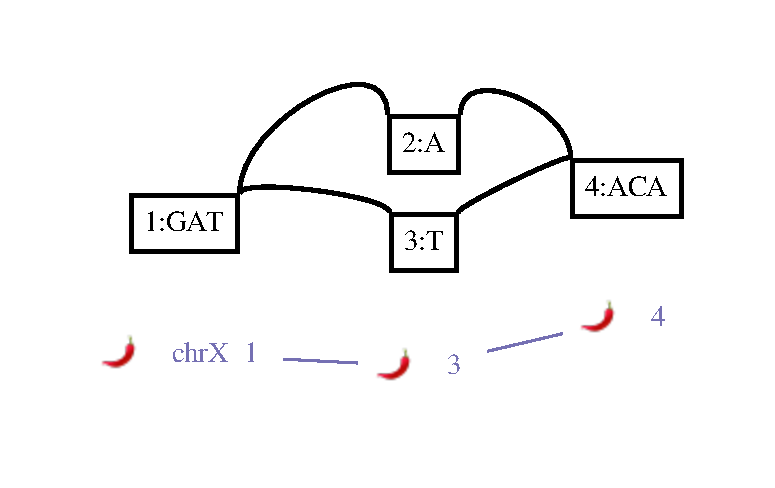
\includegraphics[width=1.10\textwidth]{fig/GRaphchrX.pdf}
\decoRule
\caption{\textbf{Fig A: Bubble}. ChrX represents the sequence used as a reference to describe variants that are present in a sequence analysed.} %aggiungere path
\label{fig:bubble.png}
\end{figure}



%%%%%%%%%%%%%%%%%%%%%%%%%%%%%%%%%%%%%%%%%%%%%%%%%%%%%%%%%%%%%%%%%%%%%%%%%%%%%%%%%%%%%%%%%%%%
%  Subsection 
%%%%%%%%%%%%%%%%%%%%%%%%%%%%%%%%%%%%%%%%%%%%%%%%%%%%%%%%%%%%%%%%%%%%%%%%%%%%%%%%%%%%%%%%%%%%


\subsection{gfa2vcf}
The gfa2vcf function converts a file from the GFA format to VCF format. Starting from the detected bubbles, a VCF file is generated.

\begin{figure}[H]
\centering
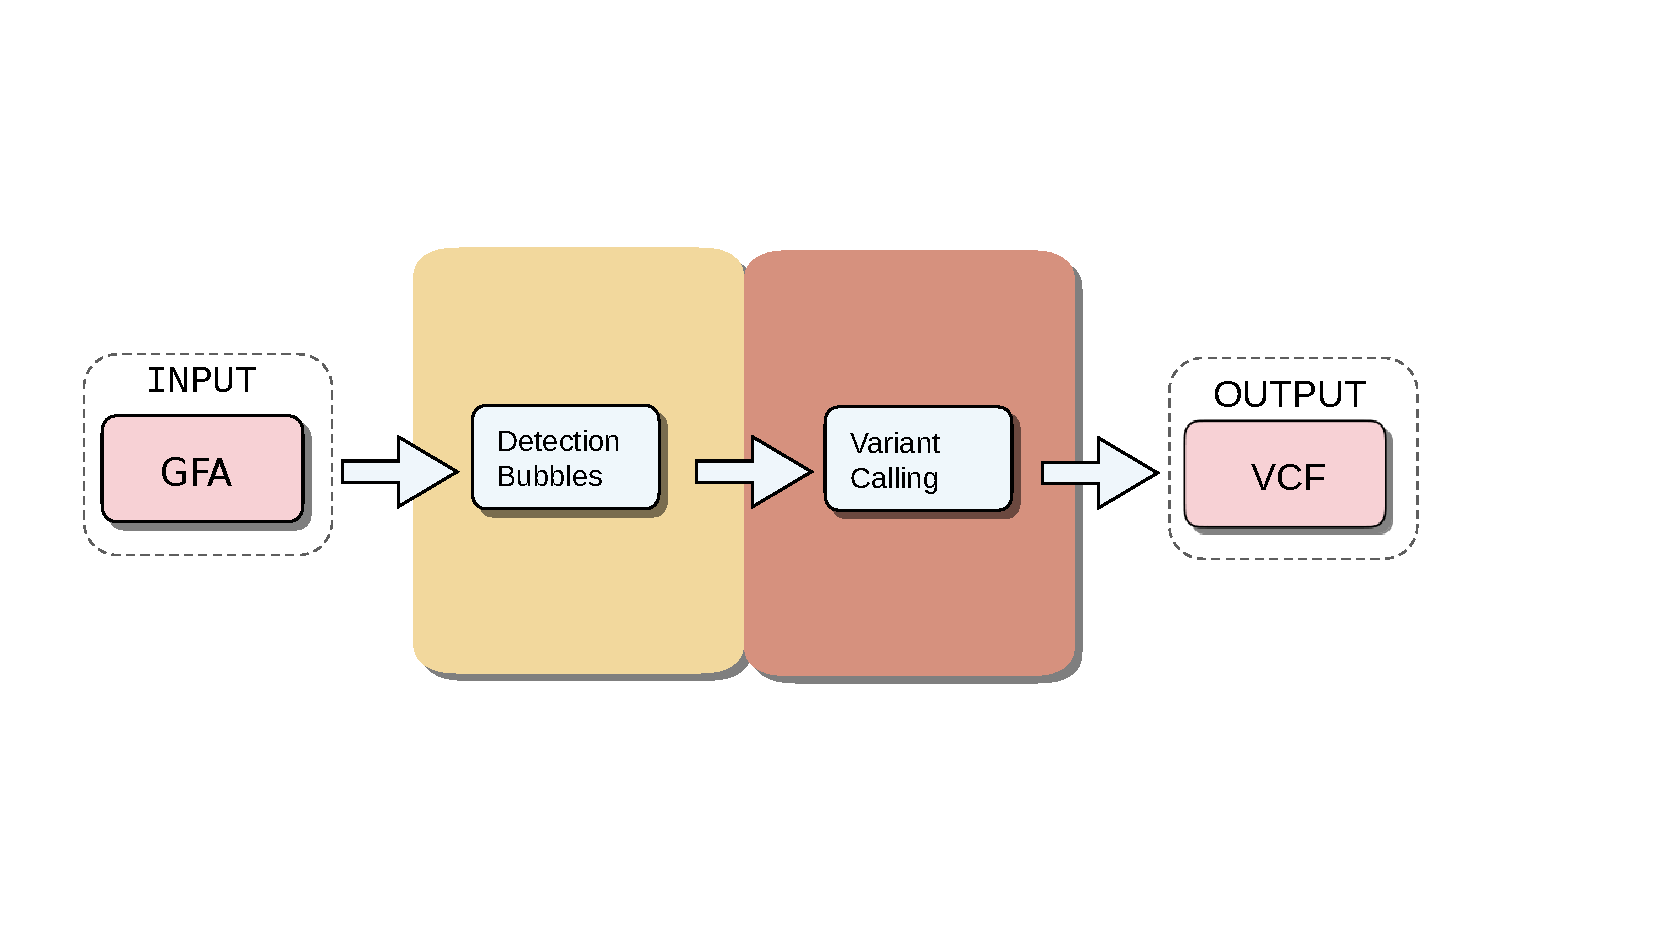
\includegraphics[width=1.10\textwidth]{fig/gfatovcf.pdf}
\decoRule
\caption{\textbf{Graph} GfatoVcf}
\label{fig:vgpop.pdf}
\end{figure}

%figura più bellina, non è inappropriato usare il termine variant calling?? CHIEDERE AD ERIK



The graph loaded using odgi (citarlo nei metodi o introduzione). 
\setcounter{secnumdepth}{3}
\subsubsection{Bubblepop} %già spiegato
\subsubsection{Extracting Variant O """QUALCOSA DEL GENERE"""}
%"""QUESTO È VARIANT CALLING, QUINDI NON VA BENE"""Variant calling is the process of identifying genetic variants. First, sequence reads from one individual are aligned against the reference genome, then variable sites are identified as the ones where the sequence differs from the reference genome.

\begin{itemize}
\item\textbf{Possible paths}
Considering all the possible paths, the variants have been called respect to a path chosen as reference. A variant is a nodes supported by at least one path, whose sequence is different from the sequence of the corresponding node in the chosen reference.

\item\textbf{SNV and INDEL}

For Deletion if the considerate node in the REF is the current node in the current path, it means that in the current path a node is missing, so there is a deletion respect to the REF.
For Insertion if the considerate node in the current path is the current node in the ref, it means that in the current path there is a node that is missing in the REF, that is an insertion.

For SNV if the sequence are different in the current path respect to the REF.
\end{itemize}


I obtained VCF.


Length of sequence in a node corresponds to	POS. POS, for example (NODE1 ATG) POS is 3 (length of sequence); for (NODE2 AT) POS is 5 because is the sum of the length of the previous node sequence plus the current node length sequence.
Chose a path (or paths) from the beginning by recording sequences, it is corresponds to REF
Sequence not present in REF, the center of bubble is ALT.

{\small
\begin{table}
\caption{Gfa to Vcf}
\label{tab:gfatovcf}
\centering
\begin{adjustbox}{width=0.50\textwidth}
\begin{tabular}{c c}
\toprule
\tabhead{GFA} & \tabhead{VCF} \\
\midrule
 Path Name & CHROM \\
 Length of sequence & POS \\
 Path Chose & REF \\
 Center of bubble & ALT \\
 SNV, INDEL & Type\\
\bottomrule\\
\end{tabular}
\end{adjustbox}
\end{table}
}
















%%%%%%%%%%%%%%%%%%%%%%%%%%%%%%%%%%%%%%%%%%%%%%%%%%%%%%%%%%%%%%%%%%%%%%%%%%%%%%%%%%%%%%%%%%%%
%  Subsubsection 
%%%%%%%%%%%%%%%%%%%%%%%%%%%%%%%%%%%%%%%%%%%%%%%%%%%%%%%%%%%%%%%%%%%%%%%%%%%%%%%%%%%%%%%%%%%%

\subsubsection{VCF and Validation}

For validation VCF:

I used vg tool (adapted from \cite{vg}) to work with genome variation graphs for validate the VCF files obtained with the gfa2vcf function. To date, the first path in the GFA file is used as reference; in the next updates, it will be possible to set any available paths.


\begin{verbatim}
./vg construct -v output.vcf.gz -r reference.fa > VcftoGraph.vg
./vg view -dp VcftoGraph.vg | dot -Tpdf -o ValidationGraph.pdf
\end{verbatim}

From these commands I obtained the graph figure ((\ref{fig:Validation.png}B)) used for validation the graph used as starting point to execute the gfa2vcf function (\ref{fig:Validation.png}A). These figures are equal, gfa2vcf works well. 



\begin{figure}[H]
\centering
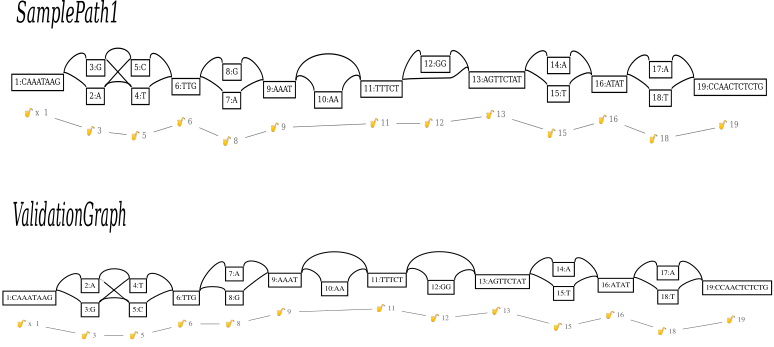
\includegraphics[width=1.10 \textwidth]{fig/Validation.png}
\decoRule
\caption{\textbf{Fig A: SamplePath}. GFA that I use to convert it to VCF 
\textbf{FigB: ValidationGraph} I use VCF to obtained from script and I obtained the same starting graph} 
\label{fig:Validation.png}
\end{figure}

%%%%%%%%%%%%%%%%%%%%%%%%%%%%%%%%%%%%%%%%%%%%%%%%%%%%%%%%%%%%%%%%%%%%%%%%%%%%%%%%%%%%%%%%%%%%
%  Subsection 
%%%%%%%%%%%%%%%%%%%%%%%%%%%%%%%%%%%%%%%%%%%%%%%%%%%%%%%%%%%%%%%%%%%%%%%%%%%%%%%%%%%%%%%%%%%%

\subsection{gfa2allelefreq} 

Allele frequency gives us indication on how common an allele is in a population. It is calculated by counting how many times the allele appears in the population, dividing by the total number of copies of the gene.

Haploids    $p = \dfrac{i}{N}$

Diploids   

frequency of A $p = {f(AA)} + \dfrac{1}{2} f(AB)$

frequency of B $q = {f(BB)} + \dfrac{1}{2} f(AB)$

Load metadata for calculate info of tree leaves (DIRLO?)

I counted ATGC in a position and I checked the reference base and calculate for each allele the frequency (count/numhaplotype).
Only allele frequencies different from 1 were considered. 
 

%%%%%%%%%%%%%%%%%%%%%%%%%%%%%%%%%%%%%%%%%%%%%%%%%%%%%%%%%%%%%%%%%%%%%%%%%%%%%%%%%%%%%%%%%%%%
%  Subsection 
%%%%%%%%%%%%%%%%%%%%%%%%%%%%%%%%%%%%%%%%%%%%%%%%%%%%%%%%%%%%%%%%%%%%%%%%%%%%%%%%%%%%%%%%%%%%


\subsection{gfa2genfreq}

Genotype frequency \cite{brooker2014principles} in a population is the number of individuals with a given genotype divided by the total number of individuals in the population. In population genetics, the genotype frequency is the frequency or proportion of genotypes in a population. 

$f(a) = \dfrac{(Aa) + 2 x (aa))}{2 x (AA) + 2 x (Aa) + 2 x (aa)}$



%%%%%%%%%%%%%%%%%%%%%%%%%%%%%%%%%%%%%%%%%%%%%%%%%%%%%%%%%%%%%%%%%%%%%%%%%%%%%%%%%%%%%%%%%%%%
%  Subsection 
%%%%%%%%%%%%%%%%%%%%%%%%%%%%%%%%%%%%%%%%%%%%%%%%%%%%%%%%%%%%%%%%%%%%%%%%%%%%%%%%%%%%%%%%%%%%


\subsection{gfa2fst}

The fixation index is a measure of population differentiation due to genetic structure. It is frequently estimated from genetic polymorphism data, such as single-nucleotide polymorphisms (SNP) or microsatellites developed as a special case of
the Wright’s fixation index ($F\textsubscript{st})$ is a measure of population differentiation due to genetic structure. 

It can be estimated as the standardized variance of allele frequencies among sub-populations.

$F\textsubscript{st} = \dfrac{s^{2}}{p(1-p)}$

with s and p being the variance and mean, respectively, of the allele frequency. 

$F\textsubscript{st}$ \cite{barbujani2010human} ranges from 0, when all sub-populations are identical, to 1, when different alleles are fixed in different sub-populations.

1. Mean of frequencies
2. Calculate Fst


\vspace{8cm}


%%%%%%%%%%%%%%%%%%%%%%%%%%%%%%%%%%%%%%%%%%%%%%%%%%%%%%%%%%%%%%%%%%%%%%%%%%%%%%%%%%%%%%%
%  Section 
%%%%%%%%%%%%%%%%%%%%%%%%%%%%%%%%%%%%%%%%%%%%%%%%%%%%%%%%%%%%%%%%%%%%%%%%%%%%%%%%%%%%%%%

\section{Application to simulated data}
I exploited analyses of genetic population on simulated data to already know what to expect.


%%%%%%%%%%%%%%%%%%%%%%%%%%%%%%%%%%%%%%%%%%%%%%%%%%%%%%%%%%%%%%%%%%%%%%%%%%%%%%%%%%%%%%%%%%%%
%  Subsection 
%%%%%%%%%%%%%%%%%%%%%%%%%%%%%%%%%%%%%%%%%%%%%%%%%%%%%%%%%%%%%%%%%%%%%%%%%%%%%%%%%%%%%%%%%%%%

\subsection{Simulation Scenario and Tools}

\subsubsection{MS}

I used MS \cite{hudson2004ms}, a program to generate samples under a variety of neutral models. The purpose of this program is to allow one to investigate the statistical properties of such samples, to evaluate estimators or statistical tests, and generally to aid in the interpretation of polymorphism data sets.

The program ms can be used to generate many independent replicate samples under a variety of assumptions about migration, recombination rate and population size. I simulated two populations that are divided into three different times. I expected Fst to be greater for the two populations more distantly divided over time.(T3)

%forse citare nei metodi pacchetto usato per fare i plot?




\begin{figure}[H]
\centering
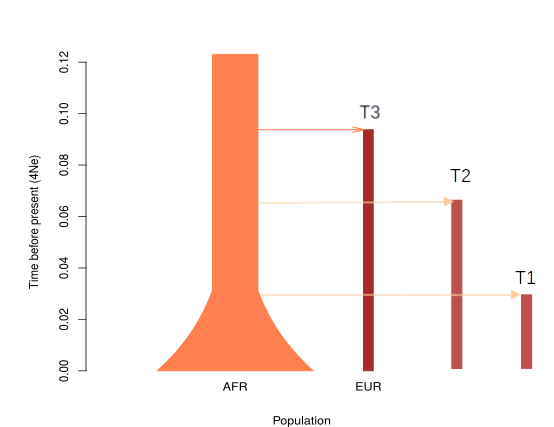
\includegraphics[width=1.10\textwidth]{fig/populationthreetime.png}
\decoRule
\caption{\textbf{Fig:Population}. 
T1 (0.031254 Ne), T2(0.0625 Ne),T3(0.09375 Ne)}
\label{fig:population.pdf}
\end{figure}

\begin{verbatim}
In the first case I simulated two populations that divided 5.000 generations ago.


ms 80 100 -t 11.2 -I 2 40 40 -g 1 44.36 -n 2 0.05 -eg 0.03125 1 0.0 -ej 0.03125 2 1   

I simulated two populations that divided 10.000 generations ago.

ms 80 100 -t 11.2 -I 2 40 40 -g 1 44.36 -n 2 0.05 -eg 0.03125 1 0.0 -ej 0.0625 2 1   

I simulated two populations that divided 15.000 generations ago.

ms 80 100 -t 11.2 -I 2 40 40 -g 1 44.36 -n 2 0.05 -eg 0.03125 1 0.0 -ej 0.09375 2 1   
\end{verbatim}

Explanation the parameters of ms:

\begin{itemize}
\item\textbf{nsam<nsample>:}
is the number of copies of the locus in each sample.

\item\textbf{nrep<nreplicate>:}
is the number of independent samples to generate;


\item\textbf{t <mutationrate>:}
is equal to $$4N0\mu$$ where N0 is the diploid population size and where u is the neutral mutation rate for the entire locus;

\item\textbf{I <individual>:}
followed by the number of subpopulations,npop, and the sample configuration. The sample configuration is a list of npop integers (n 1 n 2...) indicating the number of chromosomes sampled from each subpopulation;

\item\textbf{g <growth>:}
 it indicate the growth of pop1 at a definite time;

\item\textbf{n:}
it set growth of population 2 at time; 

\item\textbf{eg <growth rate>:}
pop1 stop growing at time 0.03125;

\item\textbf{ej <join>:}
Pop1 join with pop2. It is the parameter that change in three command. 

I convert mstogfa but I need the information about the links between the bubbles.  

\subsubsection{Seq-Gen}
I needed the whole sequence rebuilt and the links between the bubbles """SPIEGARE PERCHE' E/O PER FARCI COSA.

Seq-Gen \cite{rambaut1997seq} is a program that will simulate the evolution of nucleotide sequences along a phylogeny, using common models of the substitution process. A range of models of molecular evolution are implemented, including the general reversible model. 

Seq-Gen requires a tree as input, therefore I added the parameter -T to all the MS commands to obtained a tree as output. With seq-gen, I reconstructed the sequences for the three different simulated times.

\begin{verbatim}
seq-gen -mHKY -l 40 -s .2 -wa -z 783763255346462154 <treems40popT1> T1.seqgen

seq-gen -mHKY -l 40 -s .2 -wa -z 783763255346462154 <treems40popT2> T2.seqgen

seq-gen -mHKY -l 40 -s .2 -wa -z 783763255346462154 <treems40popT3> T3.seqgen

\end{verbatim}

Explanation of parameters:

\begin{itemize}

\item\textbf{m <MODEL>:} This option sets the model of nucleotide or amino acid substitution.
\item\textbf{l <SEQUENCELENGTH>:} This option allows the user to set the length in nucleotides or amino acids that each simulated sequence should be.
\item\textbf{s <SCALE>:} This option allows the user to set a value with which to scale the branch lengths in order to make them equal the expected number of substitutions per site for each branch. Basically Seq-Gen multiplies each branch length by this value.
\item\textbf{z <RANDOMNUMBERSEED>:} This option allows the user to specify a seed for the random number generator. Using the same seed (with the same input) will result in identical simulated datasets. This is useful because you can then delete the (often large) simulated sequence files to save disk space. To recreate a set of simulations, you must use exactly the same model options. The default is to obtain a seed from the system clock which will be displayed on the screen allowing it noted down.
\item\textbf{wa:}
Write Ancestral Sequences. This option allows the user to obtain the sequences for each of the internal nodes in the tree obtained with ms 
\end{itemize}

I converted seqgentogfa.
\end{itemize}

\subsection{Application vgpop}
\begin{figure}[H]
\centering
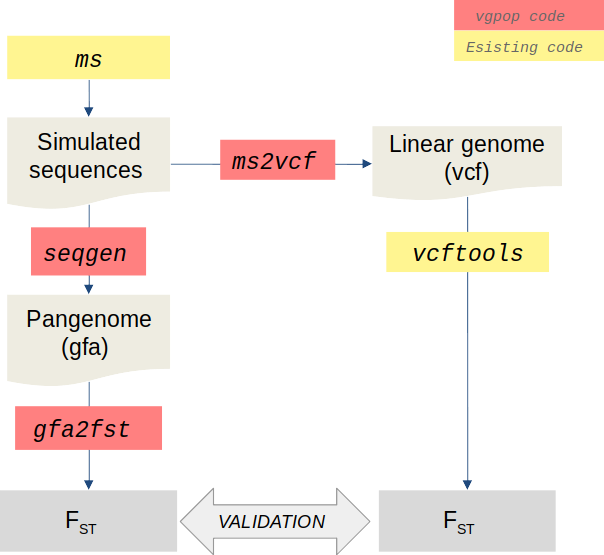
\includegraphics[width=1.00\textwidth]{fig/pipeline.png}
\decoRule
\caption{\textbf{Fig:Pipeline}. 
Validation.}
\label{fig:population.pdf}
\end{figure}

Starting from ms, I obtained simulated sequences with Seq-Gen. These sequences were encoded in a GFA file on which calculate directly the allele frequencies, the genotype frequencies, and the Fst.

For validate these result, I converted simulated sequences into a VCF file (ms2vcf), calculating the allele frequencies using vcftools. These frequencies were compared with the frequencies obtained directly from a GFA file, calculating the Fst from the VCF file and from the GFA file.


Fst is the same, I obtained major distribution from two populations that divided 15.000 years ago (time of division T3). 

(Aggiungere curva con dati combacianti, non escono identiche perchè i dati di partenza sono diversi.




\subsection{simulations works}
POTREMMO FARE COSÌ
1) mstovcf-->vcftools-->fralleliche-->fst--> simulazioni funzionano bene, t3 maggiore

\begin{figure}[H]
\centering
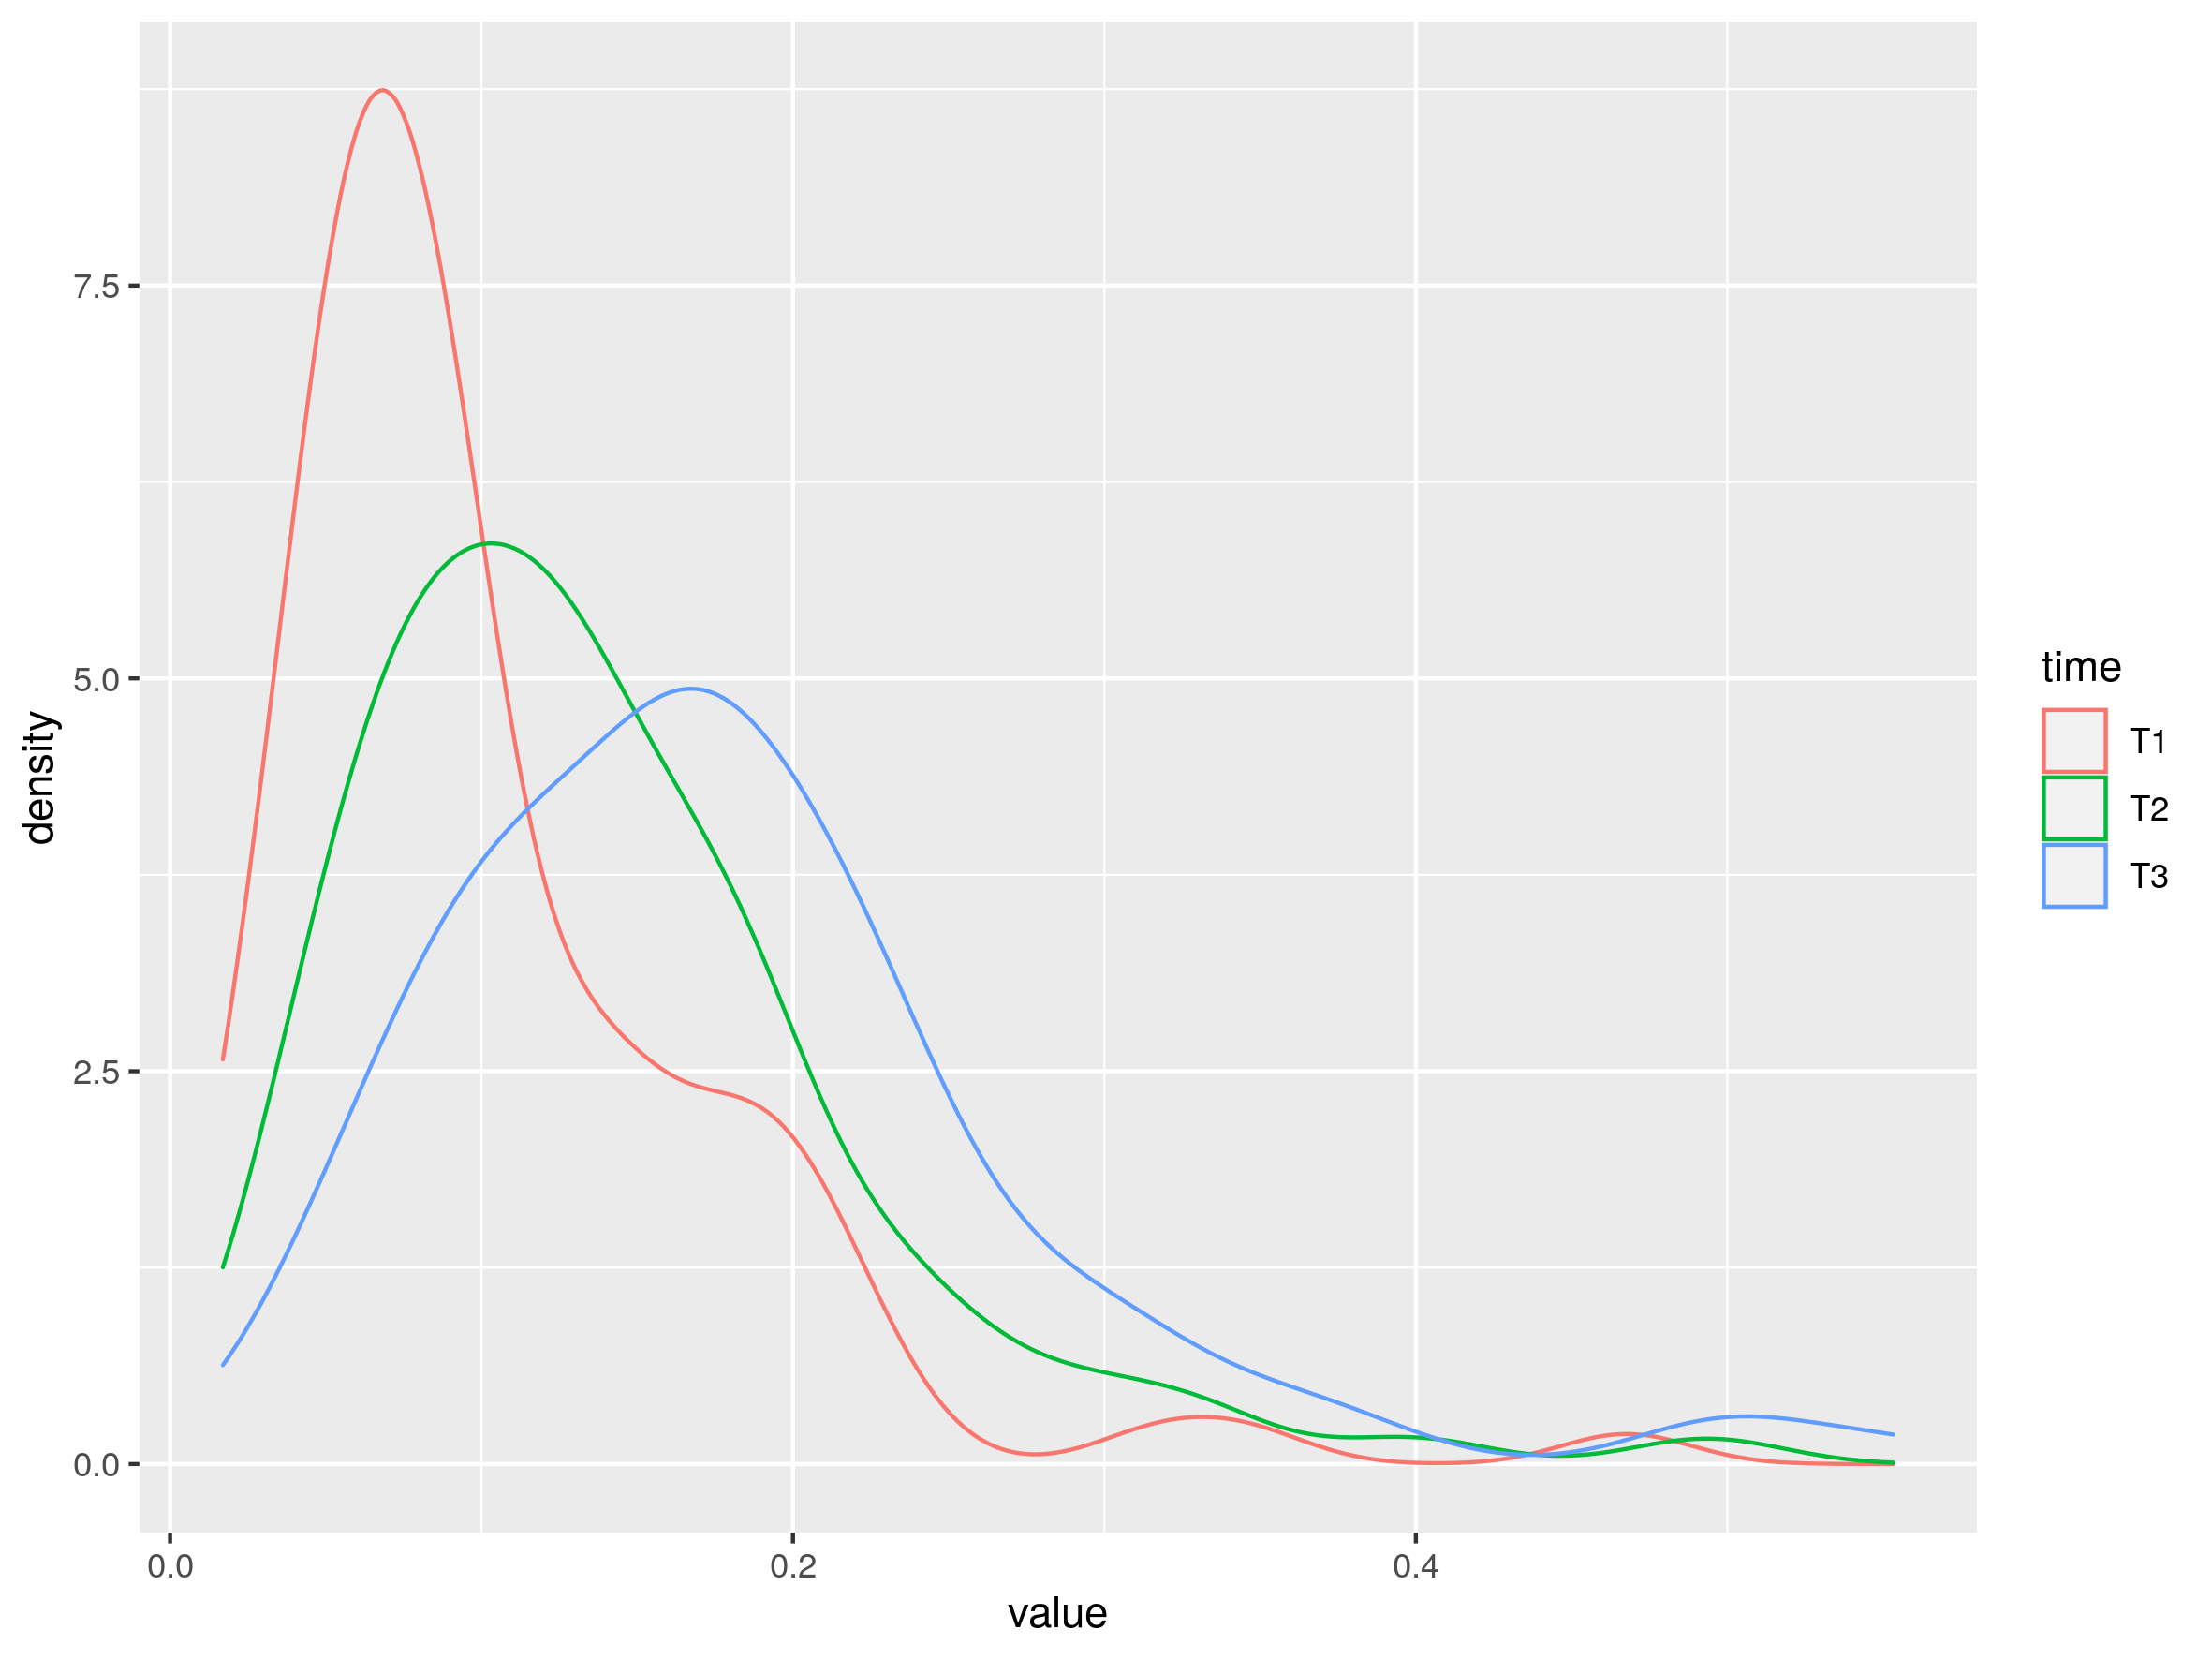
\includegraphics[width=1.00\textwidth]{fig/simulationworks.png}
\decoRule
\caption{\textbf{Fig:simulationworks}. 
Validation.}
\label{fig:simulationworks.pdf}
\end{figure}

Provato vg construct ma non dà info su tutti i path

Per avere curve identiche, due opzioni:

 
1) VCF piccolino, gfa corrispondente calcolo e vedere se escono uguali i dati per un solo locus. VALIDIAMO ANCORA  


2) mstovcf--> vcftools-->fralleliche-->fst


mstovcf-->\textit{minimap-->seqwish-->grafo}-->gfa2allelfr-->fst



3) ms-->seq-gen-->gfa-->gfa2allelfr-->fst

ms-->seq-gen-->vcf-->fralle-->fst




\section{Study Cases}

I applicate one function of \vgp to pangenomes of COVID-19 and Yeast. In particular I calculate gfa2allelefreq.

\subsection{COVID-19}

The first step is generate a pangenome from COVID-19.


\subsubsection{Pangenome}

%uso questa pipeline presente su git bh20-seq-resource. CITARE

\begin{itemize}
\item  Download sequences of Sars-Cov2 from GenBank;
\item Run a series of commands to generate a pangenome for the virus:
\end{itemize}
\begin{verbatim}

minimap2 -cx asm20 -X seqs.fa seqs.fa >seqs.paf

seqwish -s seqs.fa -p seqs.paf -g seqs.gfa

odgi build -g seqs.gfa -s -o seqs.odgi

    
\end{verbatim}













\subsection{yeast}



% Chapter discussion

\chapter{Conclusions and Future Perspectives-3/6pagine} % Main chapter title

\label{Chapter6} % For referencing the chapter elsewhere, use \ref{Chapter4} 

%----------------------------------------------------------------------------------------

% Chapter discussion

\chapter{Materials and Methods(5-10 pagine} % Main chapter title

\label{Chapter7} % For referencing the chapter elsewhere, use \ref{Chapter4} 

%----------------------------------------------------------------------------------------

%\printglossary

\printbibliography[heading=bibintoc]

\begin{acknowledgements}
\addchaptertocentry{\acknowledgementname}
\end{acknowledgements}

\end{document}